\documentclass{beamer}
\usepackage[utf8]{inputenc}
\usepackage{graphicx}
\usepackage{amsmath}
\usepackage{amssymb}
\usepackage[spanish]{babel}
\usepackage{hyperref}

\title{Modelo Matemático para la Bioconversión de Residuos y Producción de CO\textsubscript{2}}
\author{John Jairo Leal Gómez}
\date{\today}

\begin{document}

\frame{\titlepage}

\begin{frame}{Introducción}
    \begin{itemize}
        \item La mosca soldado negra (Hermetia illucens) es utilizada para la bioconversión de residuos orgánicos.
        \item Durante su desarrollo, se generan emisiones de CO\textsubscript{2} que pueden ser modeladas matemáticamente.
        \item Se emplean ecuaciones diferenciales ordinarias (EDOs) y parciales (EDPs) para predecir la dinámica de crecimiento y emisiones.
    \end{itemize}
\end{frame}

\begin{frame}{Objetivos}
    \begin{itemize}
        \item Modelar el crecimiento de la mosca soldado utilizando EDOs.
        \item Analizar la distribución espacial de CO\textsubscript{2} mediante EDPs.
        \item Evaluar la eficiencia de conversión de residuos en biomasa larval.
    \end{itemize}
\end{frame}

\begin{frame}{Modelo Matemático}
    \textbf{Ecuaciones Diferenciales:}
    \begin{itemize}
        \item Consumo de residuos:
        \begin{equation}
            \frac{dB}{dt} = -\mu_L \cdot \frac{B}{K_B + B} \cdot L
        \end{equation}
        \item Crecimiento larvario:
        \begin{equation}
            \frac{dL}{dt} = Y_{L/B} \cdot \mu_L \cdot \frac{B}{K_B + B} \cdot L \cdot \left(1 - \frac{L}{L_{\text{max}}}\right)
        \end{equation}
        \item Producción de CO\textsubscript{2}:
        \begin{equation}
            \frac{dC}{dt} = Y_{C/B} \cdot \mu_L \cdot \frac{B}{K_B + B} \cdot L
        \end{equation}
    \end{itemize}
\end{frame}

\begin{frame}{Parámetros y Variables}
    \begin{itemize}
        \item $B(t)$: Biomasa de residuos [g].
        \item $L(t)$: Biomasa larvaria [g].
        \item $C(t)$: Cantidad de CO\textsubscript{2} producida [g].
        \item $\mu_L$: Tasa máxima de consumo de residuos.
        \item $K_B$: Constante de saturación de residuos.
        \item $Y_{L/B}$: Rendimiento de biomasa larvaria.
        \item $Y_{C/B}$: Rendimiento de CO\textsubscript{2}.
    \end{itemize}
\end{frame}

\begin{frame}{Simulación en Python}
    \begin{itemize}
        \item Se resolvió el sistema de ecuaciones con el método de Runge-Kutta.
        \item Se usaron parámetros arbitrarios, aún no hay resultados experimentales.
        \item Se generaron gráficos de evolución de las variables con matplotlib.
    \end{itemize}
\end{frame}

\begin{frame}{Resultados}
    \begin{itemize}
        \item Reducción progresiva de la biomasa de residuos.
        \item Aumento de la biomasa larvaria hasta alcanzar un límite.
        \item Producción acumulativa de CO\textsubscript{2} en función del consumo de residuos.
    \end{itemize}
    \centering
    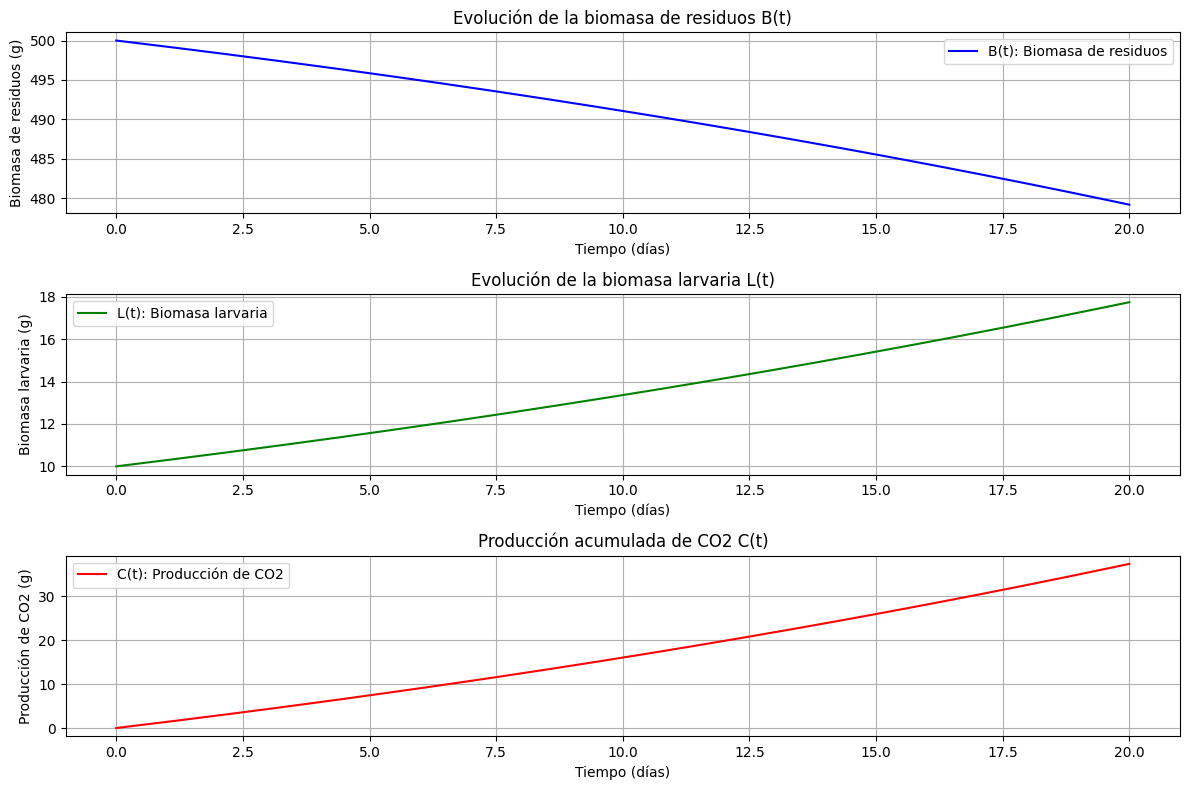
\includegraphics[width=0.8\textwidth]{solucion_ecuaciones.png} 
\end{frame}

\begin{frame}{Conclusiones}
    \begin{itemize}
        \item El modelo matemático permite predecir la conversión de residuos en biomasa larvaria y CO\textsubscript{2}.
        \item Se puede optimizar la bioconversión ajustando los parámetros del modelo.
        \item El modelo es aplicable a la gestión sostenible de residuos y producción de biomasa.
    \end{itemize}
\end{frame}

\begin{frame}{Bibliografía}
    \small
    \begin{itemize}
        \item Eriksen, N. T. (2022). "Dynamic modelling of feed assimilation, growth, lipid accumulation, and CO\textsubscript{2} production in black soldier fly larvae." PLOS ONE.
        \item Padmanabha, M. et al. (2020). "A comprehensive dynamic growth and development model of Hermetia illucens larvae.".
        \item Hansen, M. J. et al. (2023). "Metabolic performance of black soldier fly larvae during entomoremediation of biowaste." Journal of Applied Entomology.
        \item Kobelski, A. et al. (2024). "Model-based process optimization of black soldier fly egg production." Frontiers in Bioengineering and Biotechnology.
        \item Sripontan, Y. et al. (2020). "Modeling the Growth of Black Soldier Fly (Hermetia illucens)." Journal of Economic Entomology.
    \end{itemize}
\end{frame}

\end{document}
